\documentclass{article}
\usepackage{bookmark}
\usepackage{color}
\usepackage{listings}
\usepackage{amsmath}
\usepackage{hyperref}
\usepackage{listings}
\usepackage{xcolor}
\usepackage{graphicx}
\usepackage{amsfonts}
\definecolor{dkgreen}{rgb}{0,0.6,0}
\definecolor{gray}{rgb}{0.5,0.5,0.5}
\definecolor{mauve}{rgb}{0.58,0,0.82}

\lstset{
  basicstyle=\footnotesize, 
  numbers=left, 
  numberstyle=\tiny\color{gray}, 
  stepnumber=1,
  numbersep=5pt, 
  backgroundcolor=\color{white},
  showspaces=false,
  showstringspaces=false,
  showtabs=false,
  frame=shadowbox,
  rulecolor=\color{black},
  tabsize=2,
  captionpos=b,
  breaklines=true, 
  breakatwhitespace=false, 
  title=\lstname,
  keywordstyle=\color{blue},
  commentstyle=\color{dkgreen},
  escapeinside={\%*}{*)}, 
  morekeywords={*,...} 
}

\begin{document}
\begin{itemize}
\item {\bf Ex. 1}\\
{\noindent 1. The probability is $1-p^n$}, and the CPU utilization is also $1-p^n$\\

{\noindent 2. The graph is shown below:}

\begin{figure}[h]
    \centering
    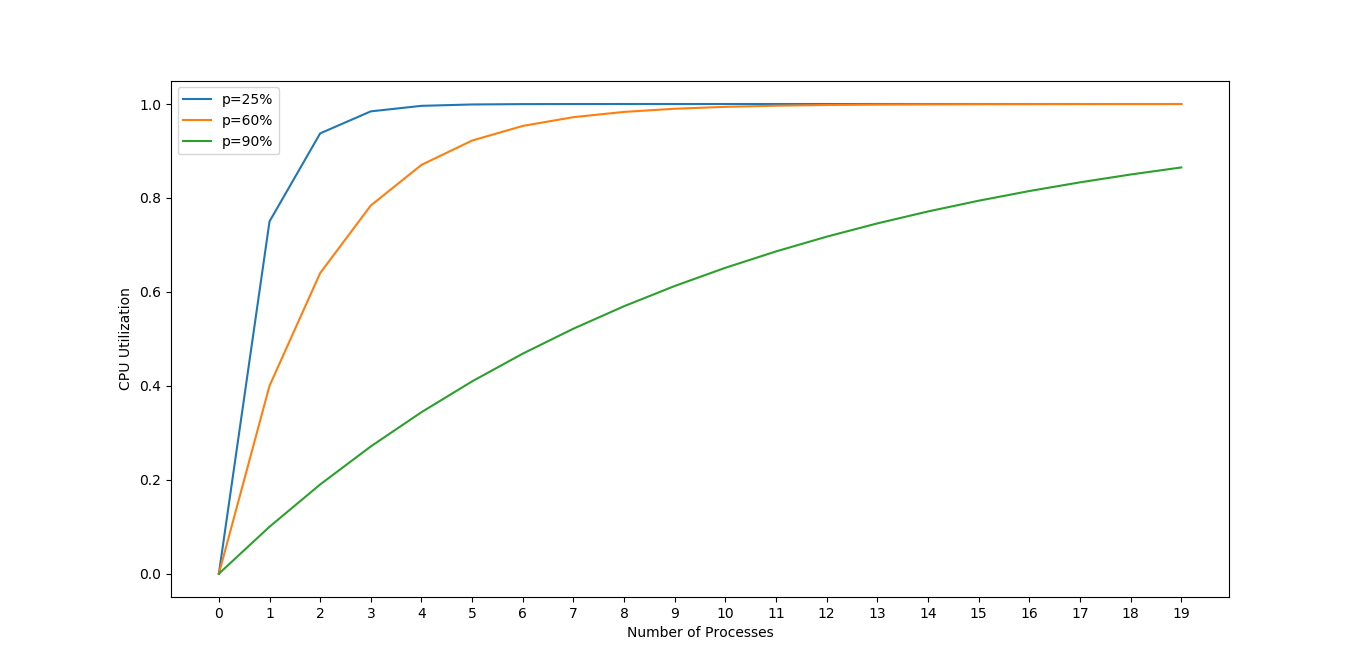
\includegraphics[scale=0.3]{1.png}
\end{figure}

{\noindent 3. (a) There can be $\lfloor \frac{256-96}{48} \rfloor =3$ processes.}\\

{\noindent (b) CPU utilization is $1-(0.9)^3=27.1\%$}\\

{\noindent (c) The result are shown below}

\begin{table}[h]
    \centering
    \begin{tabular}{|c|c|c|}
    \hline
    Adding & Number of Processes & CPU Utilization \\ \hline
    256MB  & 8                   & 56.95\%         \\ \hline
    512MB  & 14                  & 77.12\%         \\ \hline
    1024MB & 24                  & 92.02\%         \\ \hline
    \end{tabular}
\end{table}

It can be seen that adding 256MB will get the highest profit of CPU utilization improvement per MB, so it is the best.\\
\item {\bf EX. 2}\\
To accomplish this modification, those changes must be applied:\\

{\noindent 1. Go to {\color{blue} /usr/src/minix/servers/is/dmp.c}, add a line like the following. }

\begin{lstlisting}[language=C]
{ SF5,  mapping_dmp, "Print key mappings" },
{ SF6,  rproc_dmp, "Reincarnation server process table" }
{ SF7,  pronum_dmp, "Display the number of running processes"}, //added 
{ SF8,  data_store_dmp, "Data store contents" },
{ SF9,  procstack_dmp, "Processes with stack traces" },
\end{lstlisting}

{\noindent 2. Go to {\color{blue} proto.h} in the same directory, and add the following line:}

\begin{lstlisting}[language=C]
void pronum_dmp(void);
\end{lstlisting}

{\noindent 3. Go to {\color{blue} dmp\_kernel.c} and add the following function:}

\begin{lstlisting}[language=C]
void pronum_dmp(void){
        struct proc *pro;
        int r;
        if ((r=sys_getproctab(proc))!=OK){
                printf("IS: warning: couldn't get copy of process table: %d\n",r
);
                return;
        }
        int result=0;
        for (pro=BEG_PROC_ADDR;pro<END_PROC_ADDR;pro++) {
                if (!isempty(pro)) result++;
        }
        printf("There are totally %d processes\n",result);
}
\end{lstlisting}


\end{itemize}
\end{document}